\section{Lyapunov controller}
\label{sec:lyapunov_controller}

In this section, we proceed with the implementation of a Lyapunov-based controller for the already defined system.

Lyapunov control theory is a powerful tool for designing controllers that proofs the stability of non-linear systems.
The main idea is to find a Lyapunov function associated with the system and prove its convergence to the desired equilibrium point.
Notice that global asymptotic stability is guaranteed only if the Lyapunov function is positive definite and radially unbounded.

Once the Lyapunov function is defined and its properties are verified, we can derive a control law that ensures the system's stability.
Again, many methods from non-linear control theory exists such as the backstepping method, the feedback linearization method, or again passivation-based methods.

A final important remark here is that the control law derived from Lyapunov theory is not unique and generally speaking is also much more complex than the one derived from traditional linear control theory.
Even if stability is guaranteed, the performance of the system may not be optimal and a proper tuning of the controller is not always straightforward.


\subsection{Lyapunov control law}
\label{subsec:lyapunov_control_law}

Based on the work of \cite{lyapunov_techniques}, we can derive a Lyapunov control law for a generic unicycle-like system.
Given that the low level firmware of the \texttt{Turtlebot3} robot allows us to send control inputs in the form of linear and angular velocities, we can consider the turtlebot as a unicycle-like system and apply the Lyapunov control law to it.

\begin{figure}[H]
    \centering
    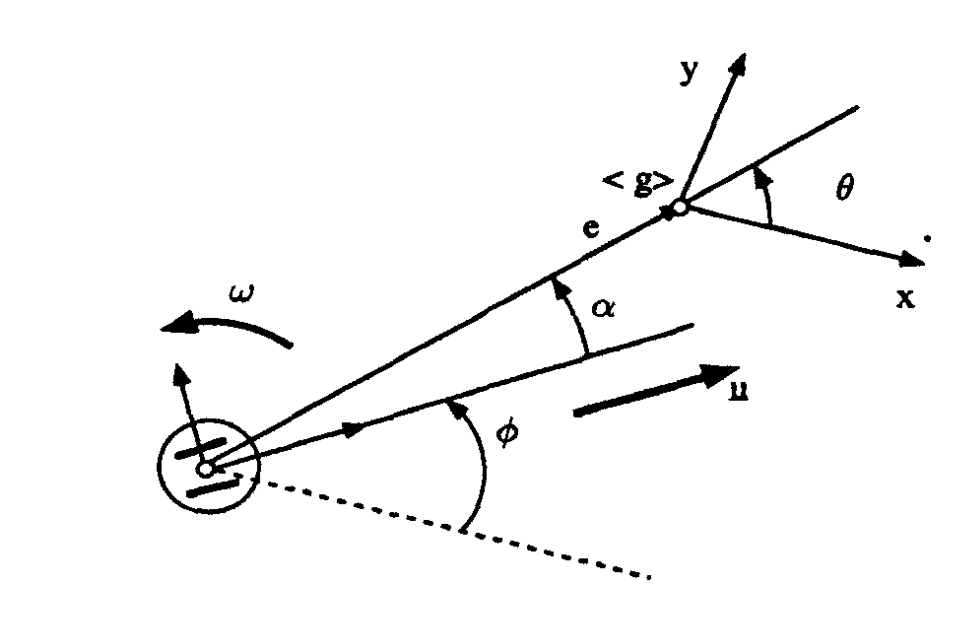
\includegraphics[width=0.7\textwidth]{./img/lyapunov_scheme.png}
    \caption{Schematic representation of the unicycle-like system and the reference frame.}
    \label{fig:lyapunov_scheme}
\end{figure}

Based on the notation used in Figure \ref{fig:lyapunov_scheme}, we can define the following Lyapunov function:

\begin{align}
    v & = k_1 \cos(\alpha) e                                                                         \\
    w & = k_2 \alpha + k_1 \frac{\sin(\alpha) \cos(\alpha)}{\alpha} \left(\alpha + k_3 \theta\right)
    \label{eq:lyapunov_control_law}
\end{align}

Where $k_1$, $k_2$, and $k_3$ are positive constants, $e$ is the Euclidean distance from the target waypoint, $\alpha$ is the angle between the robot heading and the target waypoint, and $\theta$ is the angle between the vector connecting the robot to the target waypoint and the waypoint direction (see Figure \ref{fig:lyapunov_scheme}).

It turns out that with a proper remapping of the control inputs, we can obtain a Lyapunov function that is positive definite and radially unbounded, hence ensuring the global asymptotic stability of the system.



\subsection{Implementation}
\label{subsec:lyapunov_implementation}

The code for the implementation of the Lyapunov controller is provided in the Listing \ref{lst:lyapunov_controller_code}.

\begin{lstlisting}[
    style=Matlab-editor,
    caption={Code for the implementation of the Lyapunov controller.},
    label={lst:lyapunov_controller_code}
]
function [v, w] = controlLyapunov(pos_x, pos_y, pos_yaw, target_x, target_y, target_yaw)
% This controller implements a Lyapunov-based control law for the unicycle-like
% system. It uses a Lyapunov function to derive the control inputs for the robot.
% The controller is designed to ensure global asymptotic stability of the system.
% Inspired by: Aicardi et al. (1995)

bound = @(value, limit) max(min(value, limit), -limit);

% Limits
max_linear_speed = 0.8;
max_angular_speed = 1.6;

% Gains
K_rho   = 1.0;
K_alpha = 1.5;
K_delta = 1.0;

dx = target_x - pos_x;
dy = target_y - pos_y;
rho = hypot(dx, dy);
alpha = wrapToPi(atan2(dy, dx) - pos_yaw);
theta = wrapToPi(atan2(dy, dx) - target_yaw);

% Control law (from Aicardi paper)
v = K_rho * rho * cos(alpha);
w = K_alpha * alpha + K_rho * (sin(alpha) * cos(alpha)) + K_rho * (sin(alpha) * cos(alpha)) * K_delta * theta / max(abs(alpha), 1e-3) * sign(alpha);

v = bound(v, max_linear_speed);
w = bound(w, max_angular_speed);

end
\end{lstlisting}



\subsection{Results}
\label{subsec:lyapunov_results}

The results of the obtained trajectory are shown in Figure \ref{fig:lyapunov_controller_trajectory}, where we can see the waypoints highlighted in red and the trajectory of the robot drawn in black.

\begin{figure}[H]
    \centering
    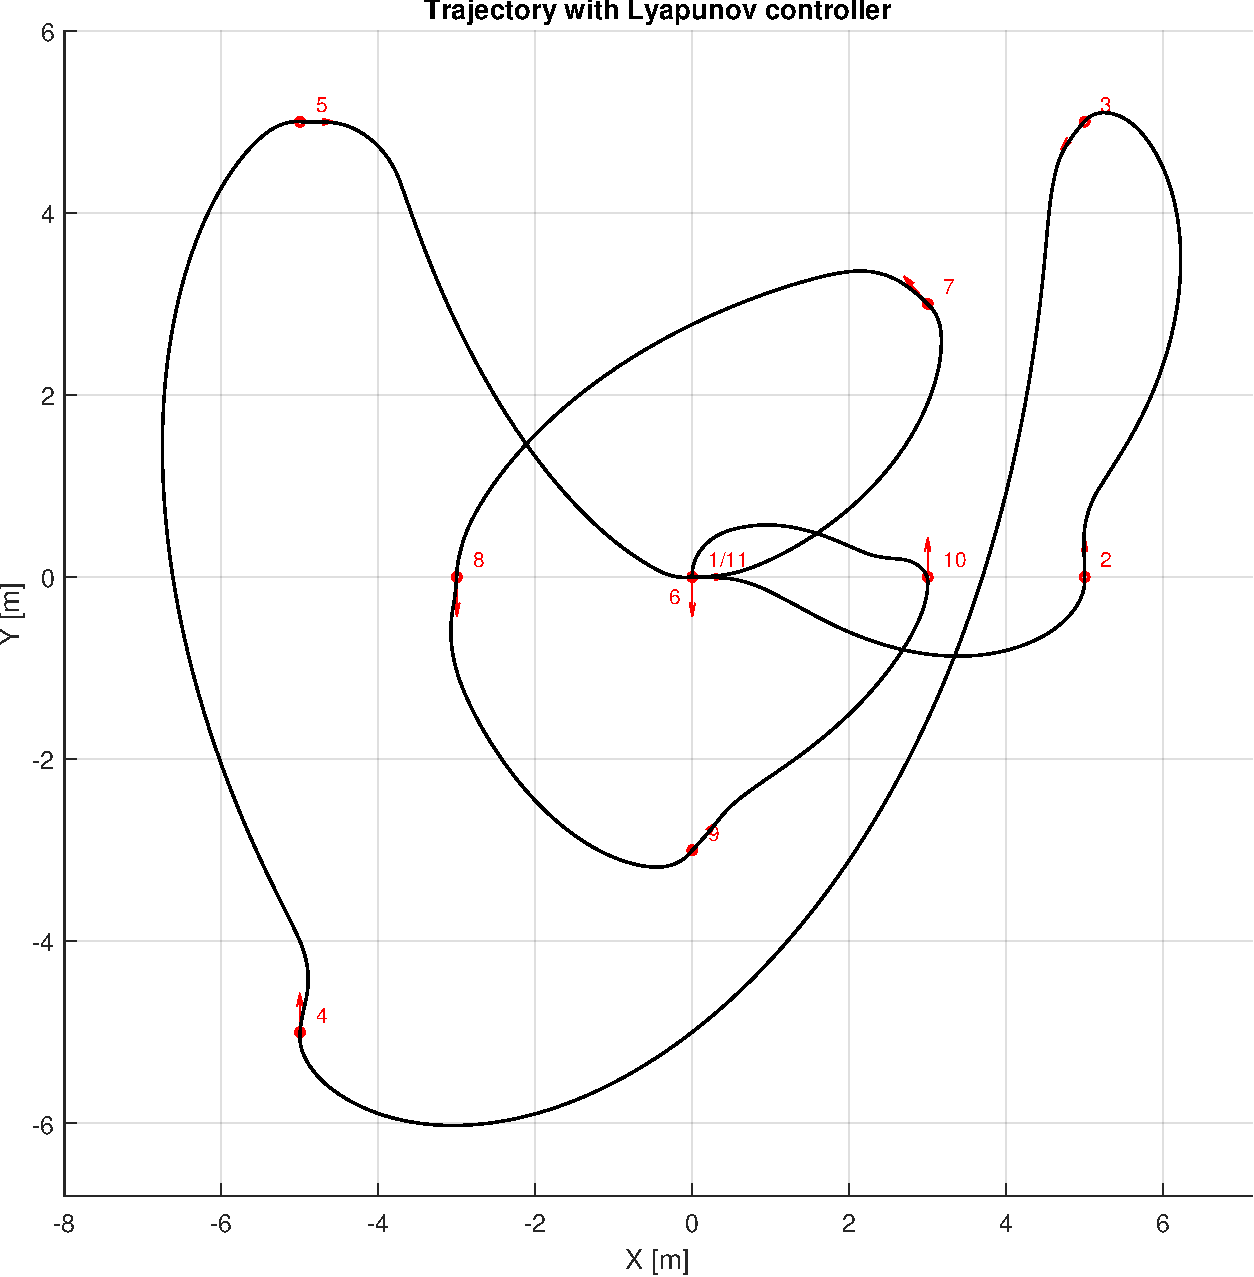
\includegraphics[width=0.6\textwidth]{./img/MATLAB/trajectory_lyapunov.pdf}
    \caption{Trajectory of the robot during the simulation with the Lyapunov controller.}
    \label{fig:lyapunov_controller_trajectory}
\end{figure}

With respect to the proportional controller, we can see that the Lyapunov controller is able to smoothly go through the waypoints and to reach them avoiding stop-and-go behavior.
The if-else logic is not needed any more given that the control law is able to smoothly connect the waypoints weighting the timing and amplitude for steering and velocity commands based on the 3 parameters $k_1$, $k_2$, and $k_3$.
One could also modify the parameters to obtain a more aggressive or conservative behavior of the robot, with consequent changes in the trajectory.

When it comes to the velocities profile, we observe that linearity is lost and non-linear behavior is present.

\begin{figure}[H]
    \centering
    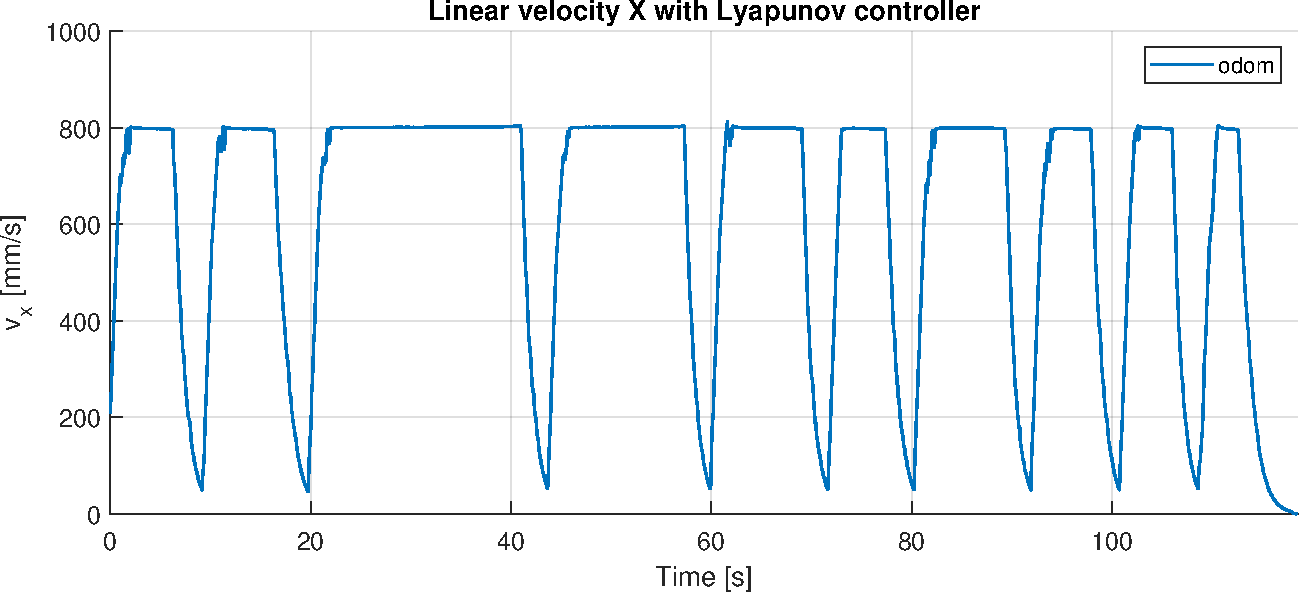
\includegraphics[width=0.7\textwidth]{./img/MATLAB/linear_velocity_lyapunov.pdf}

    \vspace{10pt}

    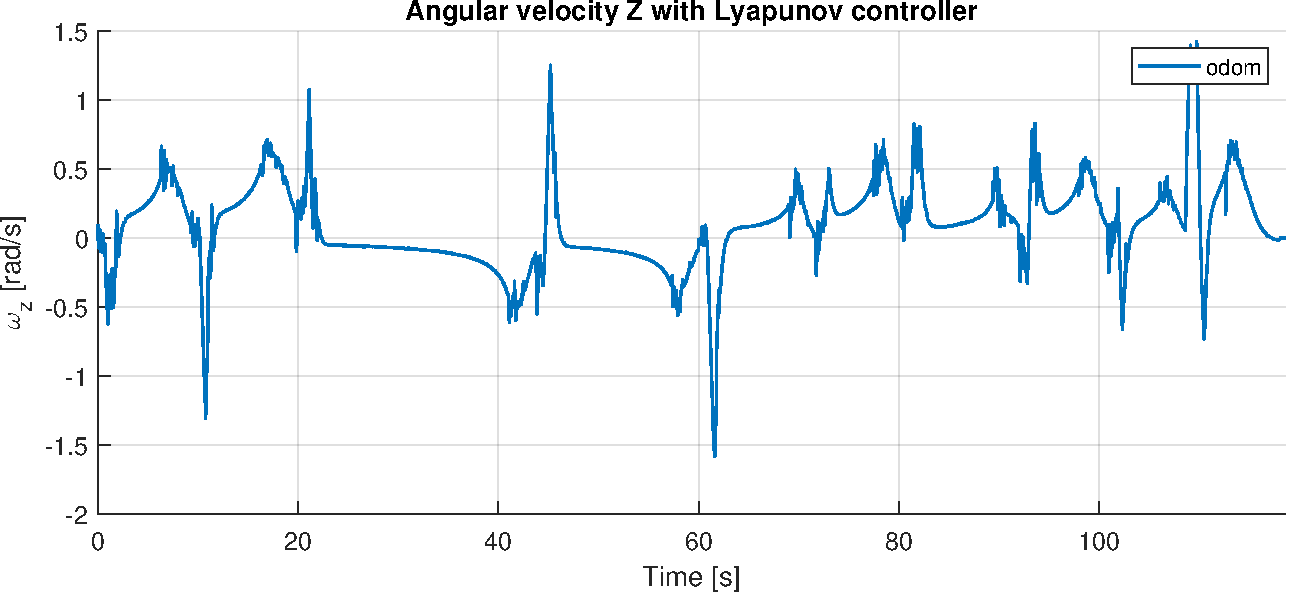
\includegraphics[width=0.7\textwidth]{./img/MATLAB/angular_velocity_lyapunov.pdf}
    \caption{Velocity profiles of the robot during the simulation with the Lyapunov controller.}
    \label{fig:lyapunov_controller_velocity_profiles}
\end{figure}

Notice that with respect to the simulation run with the proportional controller, the linear velocity is now not limited to $0.2 \text{[ m/s]}$, but it can reach up to $0.8 \text{[ m/s]}$, and similarly the angular velocity can reach up to $1.6 \text{[ rad/s]}$.
The author has decided to increase the limits of the velocities in order to allow the robot to reach the waypoints in a shorter time.
Nevertheless, the no-slip condition generally required for the unicycle-like system has been checked and verified even with the presence of stronger inertial forces due to the higher velocities.
